% -*- coding: utf-8 -*-
%-------------------------designed by zcf--------------
\documentclass[UTF8,a4paper,10pt]{ctexart}
\usepackage[left=3.17cm, right=3.17cm, top=2.74cm, bottom=2.74cm]{geometry}
\usepackage{amsmath}
\usepackage{graphicx,subfig}
\usepackage{float}
\usepackage{cite}
\usepackage{caption}
\usepackage{enumerate}
\usepackage{booktabs} %表格
\usepackage{multirow}
\newcommand{\tabincell}[2]{\begin{tabular}{@{}#1@{}}#2\end{tabular}}  %表格强制换行
%-------------------------字体设置--------------
% \usepackage{times} 
\usepackage{ctex}
\setCJKmainfont[ItalicFont=Noto Sans CJK SC Bold, BoldFont=Noto Serif CJK SC Black]{Noto Serif CJK SC}
\newcommand{\yihao}{\fontsize{26pt}{36pt}\selectfont}           % 一号, 1.4 倍行距
\newcommand{\erhao}{\fontsize{22pt}{28pt}\selectfont}          % 二号, 1.25倍行距
\newcommand{\xiaoer}{\fontsize{18pt}{18pt}\selectfont}          % 小二, 单倍行距
\newcommand{\sanhao}{\fontsize{16pt}{24pt}\selectfont}  %三号字
\newcommand{\xiaosan}{\fontsize{15pt}{22pt}\selectfont}        % 小三, 1.5倍行距
\newcommand{\sihao}{\fontsize{14pt}{21pt}\selectfont}            % 四号, 1.5 倍行距
\newcommand{\banxiaosi}{\fontsize{13pt}{19.5pt}\selectfont}    % 半小四, 1.5倍行距
\newcommand{\xiaosi}{\fontsize{12pt}{18pt}\selectfont}            % 小四, 1.5倍行距
\newcommand{\dawuhao}{\fontsize{11pt}{11pt}\selectfont}       % 大五号, 单倍行距
\newcommand{\wuhao}{\fontsize{10.5pt}{15.75pt}\selectfont}    % 五号, 单倍行距
%-------------------------章节名----------------
\usepackage{ctexcap} 
\CTEXsetup[name={,、},number={ \chinese{section}}]{section}
\CTEXsetup[name={(,)},number={\chinese{subsection}}]{subsection}
\CTEXsetup[name={,.},number={\arabic{subsubsection}}]{subsubsection}
%-------------------------页眉页脚--------------
\usepackage{fancyhdr}
\pagestyle{fancy}
\lhead{\kaishu \leftmark}
% \chead{}
\rhead{\kaishu 并行程序设计实验报告}%加粗\bfseries 
\lfoot{}
\cfoot{\thepage}
\rfoot{}
\renewcommand{\headrulewidth}{0.1pt}  
\renewcommand{\footrulewidth}{0pt}%去掉横线
\newcommand{\HRule}{\rule{\linewidth}{0.5mm}}%标题横线
\newcommand{\HRulegrossa}{\rule{\linewidth}{1.2mm}}
%-----------------------伪代码------------------
\usepackage{algorithm}  
\usepackage{algorithmicx}  
\usepackage{algpseudocode}  
\floatname{algorithm}{Algorithm}  
\renewcommand{\algorithmicrequire}{\textbf{Input:}}  
\renewcommand{\algorithmicensure}{\textbf{Output:}} 
\usepackage{lipsum}  
\makeatletter
\newenvironment{breakablealgorithm}
  {% \begin{breakablealgorithm}
  \begin{center}
     \refstepcounter{algorithm}% New algorithm
     \hrule height.8pt depth0pt \kern2pt% \@fs@pre for \@fs@ruled
     \renewcommand{\caption}[2][\relax]{% Make a new \caption
      {\raggedright\textbf{\ALG@name~\thealgorithm} ##2\par}%
      \ifx\relax##1\relax % #1 is \relax
         \addcontentsline{loa}{algorithm}{\protect\numberline{\thealgorithm}##2}%
      \else % #1 is not \relax
         \addcontentsline{loa}{algorithm}{\protect\numberline{\thealgorithm}##1}%
      \fi
      \kern2pt\hrule\kern2pt
     }
  }{% \end{breakablealgorithm}
     \kern2pt\hrule\relax% \@fs@post for \@fs@ruled
  \end{center}
  }
\makeatother
%------------------------代码-------------------
\usepackage{xcolor} 
\usepackage{listings} 
\lstset{ 
breaklines,%自动换行
language=C++,
basicstyle=\small,
escapeinside=``,
keywordstyle=\color{ blue!70} \bfseries,
commentstyle=\color{red!50!green!50!blue!50},% 
stringstyle=\ttfamily,% 
extendedchars=false,% 
linewidth=\textwidth,% 
numbers=left,% 
numberstyle=\tiny \color{blue!50},% 
frame=trbl% 
rulesepcolor= \color{ red!20!green!20!blue!20} 
}
%------------超链接----------
\usepackage[colorlinks,linkcolor=black,anchorcolor=blue]{hyperref}
%------------------------TODO-------------------
\usepackage{enumitem,amssymb}
\newlist{todolist}{itemize}{2}
\setlist[todolist]{label=$\square$}
% for check symbol 
\usepackage{pifont}
\newcommand{\cmark}{\ding{51}}%
\newcommand{\xmark}{\ding{55}}%
\newcommand{\done}{\rlap{$\square$}{\raisebox{2pt}{\large\hspace{1pt}\cmark}}\hspace{-2.5pt}}
\newcommand{\wontfix}{\rlap{$\square$}{\large\hspace{1pt}\xmark}}
%------------------------水印-------------------
\usepackage{tikz}
\usepackage{xcolor}
\usepackage{eso-pic}

\newcommand{\watermark}[3]{\AddToShipoutPictureBG{
\parbox[b][\paperheight]{\paperwidth}{
\vfill%
\centering%
\tikz[remember picture, overlay]%
  \node [rotate = #1, scale = #2] at (current page.center)%
    {\textcolor{gray!80!cyan!30!magenta!30}{#3}};
\vfill}}}

\usepackage{framed} %框框

%———————————————————————————————————————————正文———————————————————————————————————————————————
%----------------------------------------------
\begin{document}
\begin{titlepage}
    \begin{center}
    
\includegraphics[width=0.8\textwidth]{NKU.png}\\[1cm]    
    \textsc{\Huge \kaishu{\textbf{南\ \ \ \ \ \ 开\ \ \ \ \ \ 大\ \ \ \ \ \ 学}} }\\[0.9cm]
    \textsc{\huge \kaishu{\textbf{计\ \ 算\ \ 机\ \ 学\ \ 院}}}\\[0.5cm]
    \HRule \\[0.9cm]
    { \LARGE \bfseries 招聘网站项目文档}\\[0.4cm]
    \HRule \\[2.0cm]
    \centering
    \textsc{\LARGE 王\ \ 浩\ \ 2013287}\\[0.5cm]
    \textsc{\LARGE 王照钦\ \ 1911484}\\[0.5cm]
    \textsc{\LARGE 王昕炜\ \ 2113426}\\[0.5cm]
    \textsc{\LARGE 张麟浩\ \ 2113976}\\[0.5cm]
    \textsc{\LARGE 李铭辉\ \ 2011266}\\[0.5cm]
    % \textsc{\LARGE \kaishu{年级\ :\ 2020级}}\\[0.5cm]
    % \textsc{\LARGE \kaishu{专业\ :\ 信息与计算科学}}\\[0.5cm]
    \textsc{\LARGE \kaishu{指导老师\ :\ 李起成}}\\[0.5cm]
    \vfill
    {\Large \today}
    \end{center}
\end{titlepage}


%----------------------------------------------------------------
\tableofcontents
%----------------------------------------------------------------
\newpage
\watermark{60}{10}{NKU}
\setcounter{page}{1}


\section{小组个人信息}


组长:王浩(2013287)  
组员:王照钦(1911484)  
组员:王昕炜(2113426)  
组员:张麟浩(2113976)  
组员:李铭辉(2011266)  

备注:均为 0930 李起成老师班级。


\section{项目概况}
\subsection{任务目标}

本招聘网站项目的主要目标包括:

\begin{enumerate}
    \item \textbf{用户注册与登录}:实现用户(求职者和招聘方)注册、登录、以及账户管理功能,包括用户信息的增删改查。
    \item \textbf{职位发布与管理}:招聘方可以发布和管理职位信息,包括职位的分类、描述、要求等,并能够编辑和删除职位。
    \item \textbf{求职功能}:求职者可以浏览、搜索并申请职位,并能够查看申请状态和历史记录。
    \item \textbf{简历管理}:求职者可以创建、编辑简历。
    \item \textbf{通知与消息}:系统提供通知功能,向用户推送招聘进展、面试安排等消息,同时提供站内消息功能,方便用户之间的交流。
    \item \textbf{推荐系统}:实现职位推荐和简历推荐功能,帮助招聘方和求职者更快匹配合适的工作和人才。
    \item \textbf{安全性与隐私保护}:保证用户数据的安全性和隐私保护,采用加密算法进行数据存储,防止数据泄露和滥用。
    \item \textbf{用户体验}:提供良好的用户界面和用户体验,使用户能够方便快捷地完成所有操作。
\end{enumerate}

\subsection{用户特点}
本系统的最终用户主要分为三类:求职者、招聘方和管理员。

\begin{itemize}
    \item [\textbf{求职者}]
    \begin{itemize}
        \item 注册并创建个人账号。
        \item 浏览和搜索职位信息。
        \item 投递简历和查看申请进度。
        \item 接收面试通知和系统推荐的职位信息。
    \end{itemize}
    \item [\textbf{招聘方}] 
    \begin{itemize}
        \item 注册并创建公司账号。
        \item 发布和管理招聘职位。
        \item 浏览和筛选求职者简历。
        \item 通知求职者面试安排和录用信息。
    \end{itemize}
    \item [\textbf{管理员}]  
    \begin{itemize}
        \item 系统的整体管理与维护。
        \item 管理用户账号,包括求职者和招聘方的注册申请审核、账号启用和禁用。
        \item 监控系统运行状态,确保系统稳定和安全。
        \item 审核和管理招聘信息,确保职位信息的合法性和真实性。
        \item 处理用户反馈和投诉,提供技术支持。
        \item 生成系统报告和统计数据,提供给决策层参考。
    \end{itemize}
\end{itemize}

\section{假定与约束}

\begin{enumerate}
    \item 系统运行的最小寿命:在无重大改动的情况下运行 3 年。
    \item 开发期限:120 天。
    \item 假设相关硬件设备齐全。
    \item 假设系统相关功能达到预期要求。
    \item 系统必须遵守数据保护和隐私法规,支持高并发访问,确保在用户高峰期依然能够稳定运行。
    \item 系统需要满足网络安全和信息安全的相关规定和要求,包括但不限于防止黑客攻击、数据泄露等方面的规定。
\end{enumerate}

\section{需求分析}

\subsection{业务描述}

\subsubsection{系统总业务流程图及其描述}

\begin{figure}[H]
    \centering
    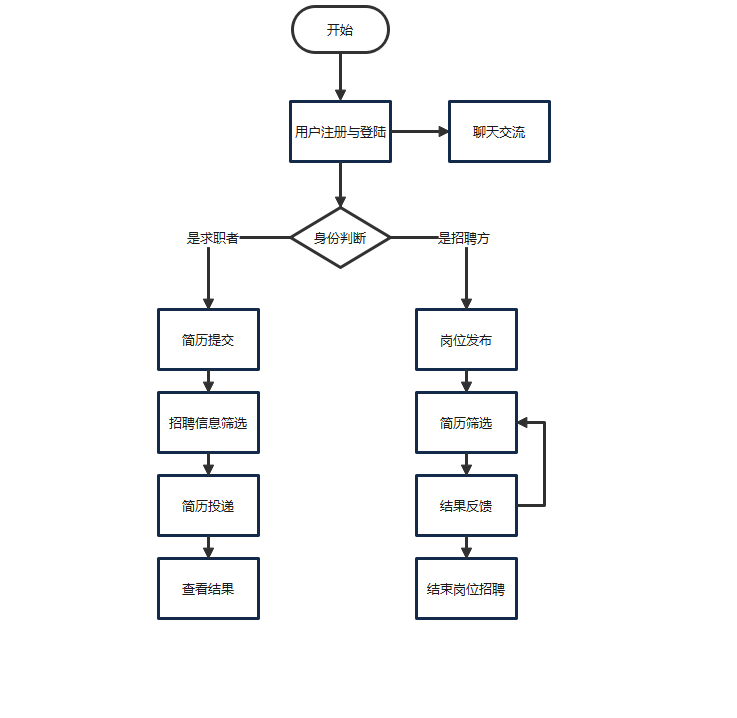
\includegraphics[width=\textwidth]{img/总业务流程图.png}
    \caption{总业务流程图}
    \label{fig:总业务流程图}
\end{figure}

总业务流程图\ref{fig:总业务流程图}概述了招聘平台的核心操作流程。用户首先在平台上注册并登录,随后根据其身份(求职者或招聘方)进入不同的操作路径。求职者可以提交简历并根据个人条件筛选并申请职位,而招聘方则负责发布岗位需求并对收到的简历进行筛选。双方通过平台进行互动,求职者投递简历后,招聘方会根据岗位要求进行评估并给出反馈。这个过程不断进行,直到招聘方找到合适的候选人并结束岗位的招聘。此外,无论用户是求职者还是招聘方,都可以在聊天系统与他人交流、分享职位信息。

\subsubsection{各个子业务流程图及其描述}

\begin{figure}[H]
    \centering
    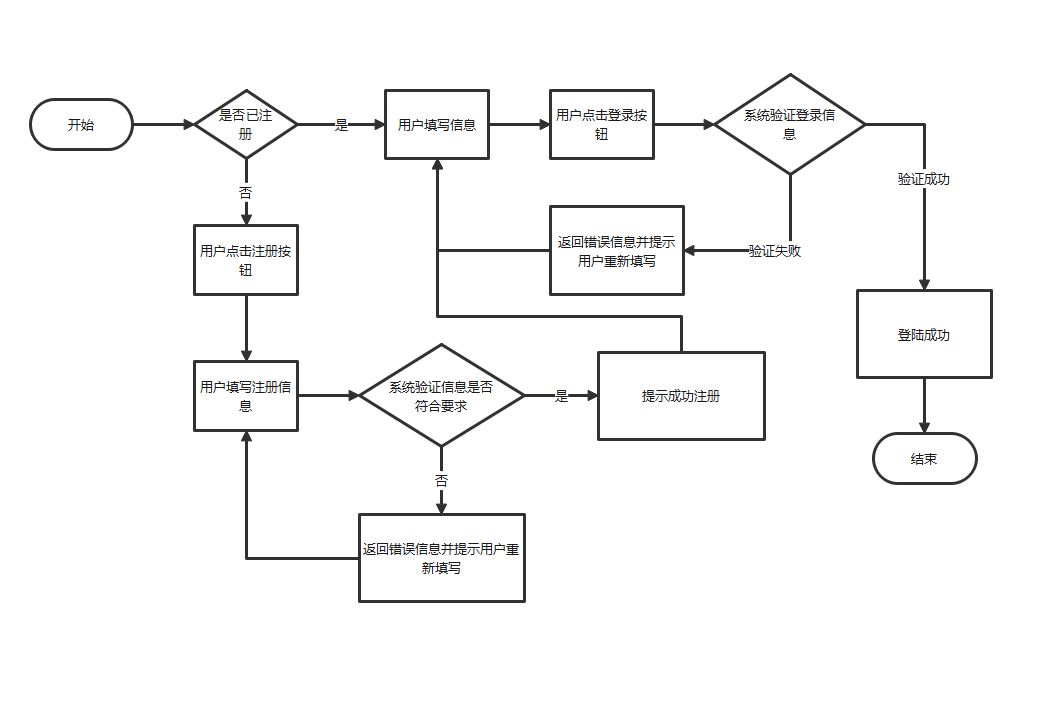
\includegraphics[width=\textwidth]{img/登陆子流程图.png}
    \caption{注册登录子流程图}
    \label{fig:注册登录子流程图}
\end{figure}

\textbf{(1)注册登录} \\注册登录子流程图\ref{fig:注册登录子流程图}展示了用户在进行登录和注册操作时的系统响应流程。当用户访问系统时,首先需要自行判断是否已经注册。如果已注册,用户将点击登录按钮并输入个人信息,系统随后验证这些信息。如果登录信息正确,用户将成功登录;如果不正确,系统会提示错误并要求用户重新填写。对于未注册的用户,他们将选择注册按钮并填写注册信息。系统将检查这些信息是否符合注册要求,如果符合,用户将被告知注册成功;如果不符合,系统同样会返回错误信息并要求用户重新填写。

\textbf{(2)求职者} \\
\begin{figure}[H]
    \centering
    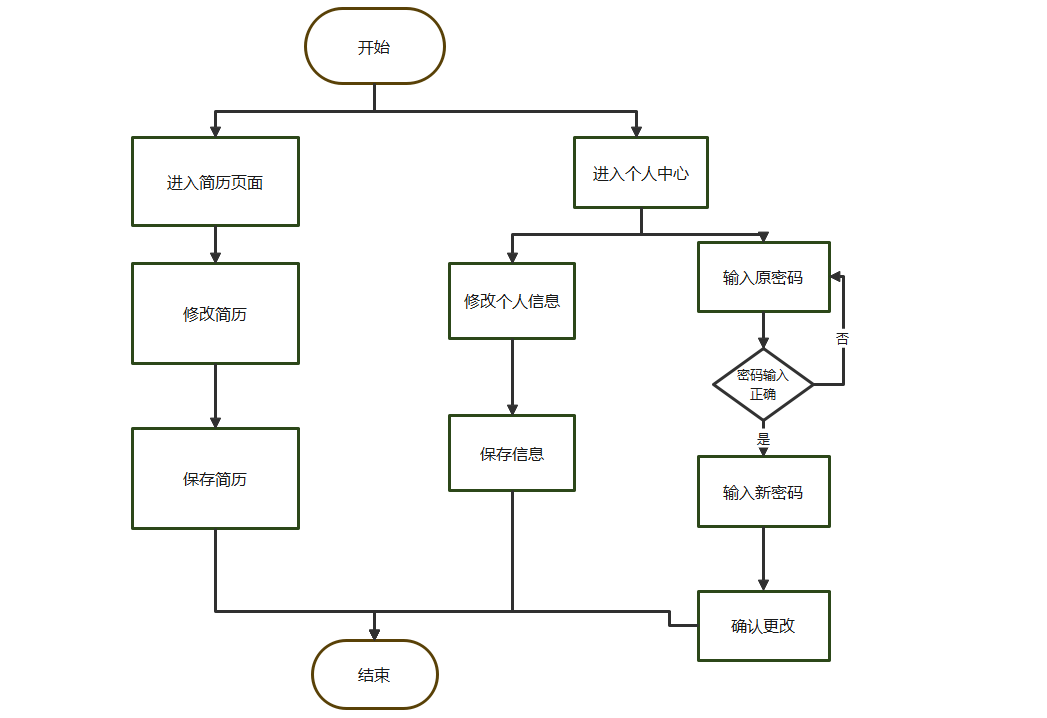
\includegraphics[width=\textwidth]{img/求职者个人信息管理.png}
    \caption{求职者个人信息管理}
    \label{fig:求职者个人信息管理}
\end{figure}

\textbf{个人信息管理与简历编辑}\space 在求职者登陆后,可以进入个人中心,修改姓名、性别等个人信息。也可以进入修改密码界面,输入原密码确认成功后,可以输入新密码并确认密码,确认更改后保存新密码。此外,还可以访问简历编辑页面,编辑个人简历并保存。
\begin{figure}[H]
    \centering
    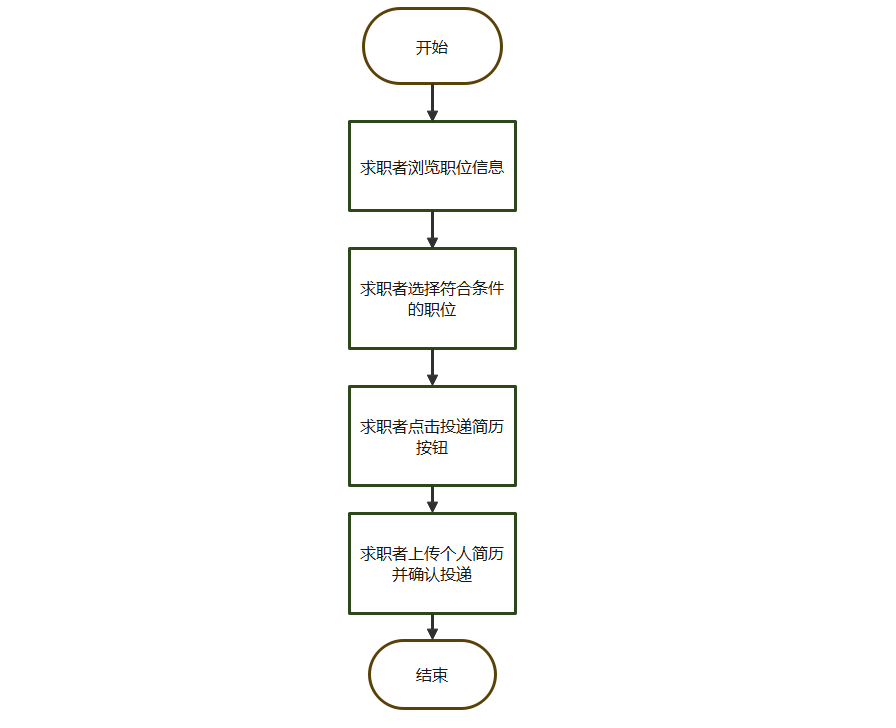
\includegraphics[width=\textwidth]{img/简历投递子流程.png}
    \caption{简历投递子流程}
    \label{fig:简历投递子流程}
\end{figure}

\textbf{投递简历}\space 求职者首先浏览各种职位信息,寻找与自己资质和兴趣相匹配的岗位。一旦找到合适的职位,他们会点击投递简历的按钮,随后确认投递自己的个人简历。一旦投递完成,流程即告结束,求职者的简历便会被发送至招聘方进行审核。

\textbf{(3)招聘方} \\
\begin{figure}[H]
    \centering
    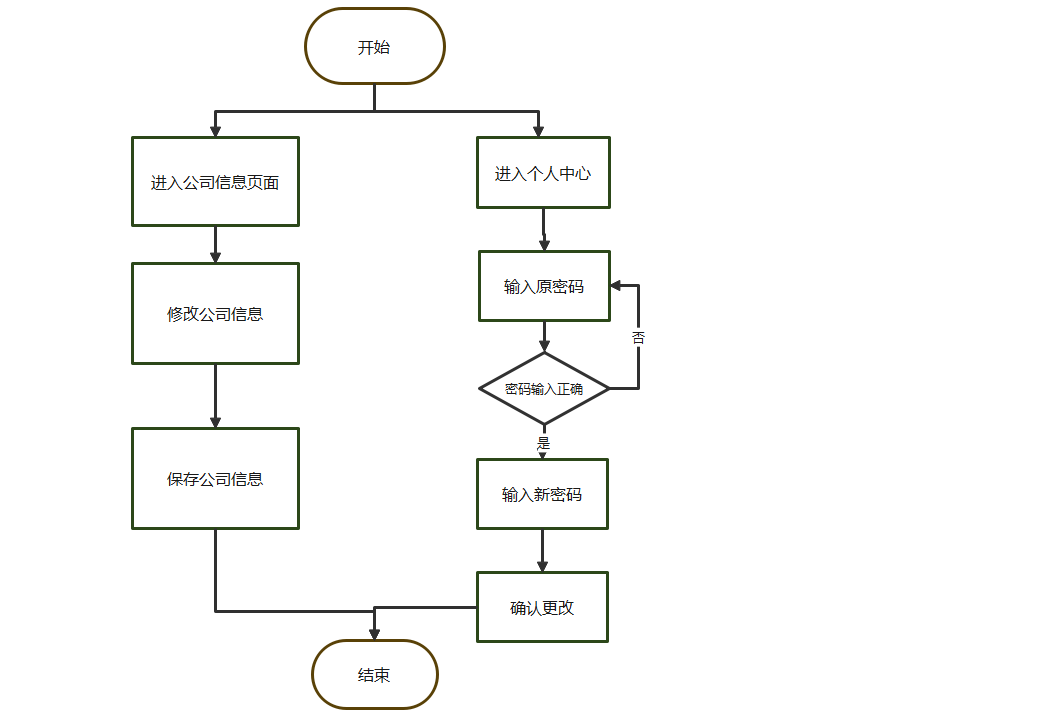
\includegraphics[width=\textwidth]{img/招聘方个人信息管理.png}
    \caption{招聘方个人信息管理}
    \label{fig:招聘方个人信息管理}
\end{figure}

\textbf{个人信息管理}\space 在招聘方登陆后,可以进入个人中心,修改密码,输入原密码确认成功后,可以输入新密码并确认密码,确认更改后保存新密码。此外,还可以访问公司信息编辑页面,编辑公司信息并保存。

\begin{figure}[H]
    \centering
    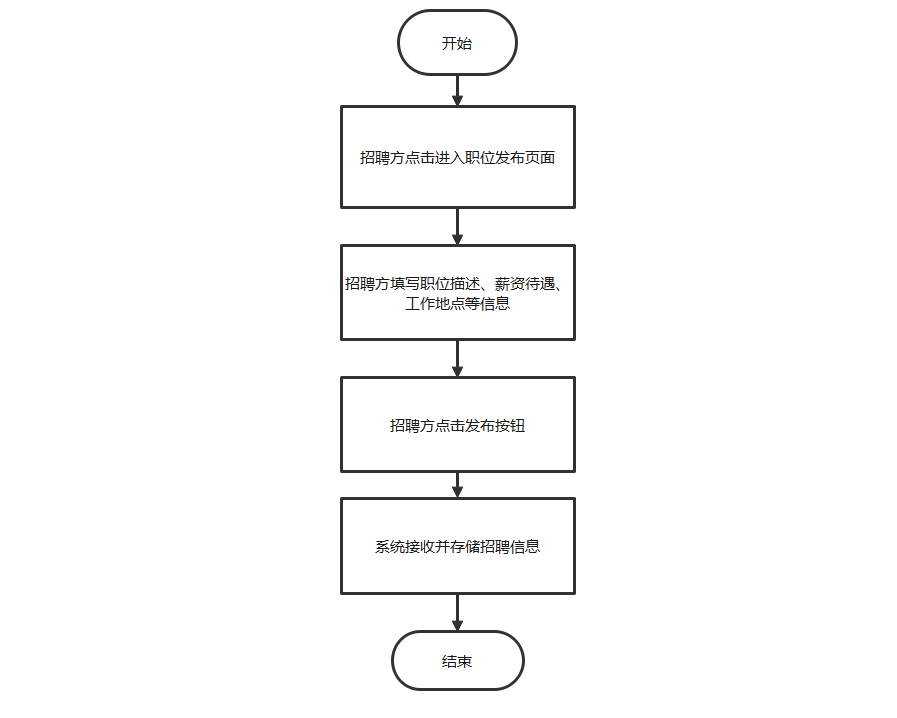
\includegraphics[width=\textwidth]{img/招聘信息发布子流程.png}
    \caption{招聘信息发布子流程}
    \label{fig:招聘信息发布子流程}
\end{figure}

\textbf{职位发布}\space 招聘方首先进入职位发布页面,然后详细填写包括职位描述、薪资待遇和工作地点在内的关键信息。点击发布按钮后,系统便会自动接收并存储这些信息。

\begin{figure}[H]
    \centering
    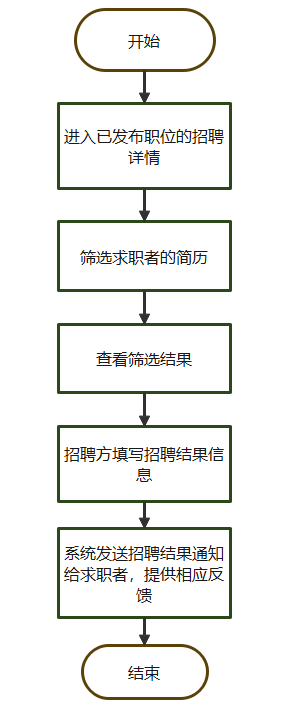
\includegraphics[width=100pt]{img/招聘结果反馈子流程.png}
    \caption{招聘结果反馈子流程}
    \label{fig:招聘结果反馈子流程}
\end{figure}

\textbf{招聘结果反馈}\space 招聘方选择要查看详情的已发布职位,然后查看求职者的简历,然后填写相应的招聘结果反馈信息,例如录取、拒绝、进一步面试安排等。系统随后自动发送这些信息给求职者,并提供反馈,确保求职者及时了解申请结果。

\begin{figure}[H]
    \centering
    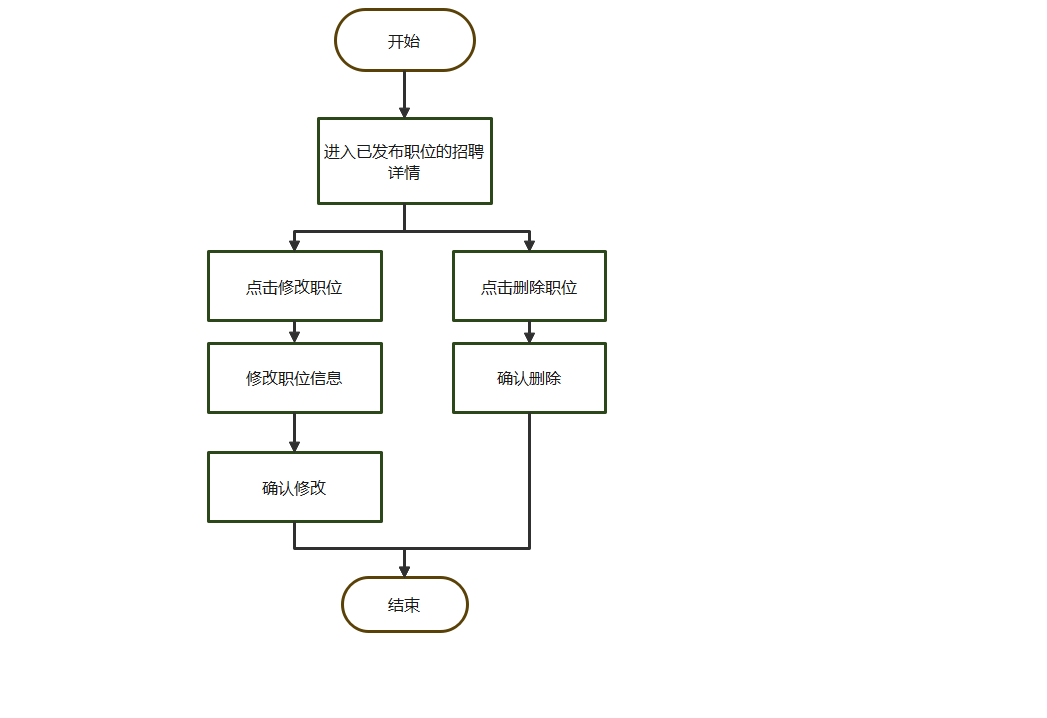
\includegraphics[width=\textwidth]{img/已发布职位管理.png}
    \caption{已发布职位管理}
    \label{fig:已发布职位管理}
\end{figure}

\textbf{管理已发布职位}\space 招聘方首先进入系统查看已发布的职位列表,然后选择需要操作的职位。如果需要修改职位信息,点击修改按钮,进入编辑页面进行编辑,并在完成后确认修改。如果招聘方决定删除某个职位,则点击删除按钮,系统会弹出确认对话框以避免误操作。一旦招聘方确认删除或修改,流程结束,职位信息将相应地更新或从系统中移除。

\subsection{数据需求}

\subsubsection{数据需求描述}

\begin{enumerate}
    \item 用户(包括求职者、招聘方)信息,用于满足用户浏览和修改个人信息的需求。
    \item 职位信息,用于用户查看职位。
    \item 求职信息,用于满足求职者投递简历、招聘方查看求职者简历的需求。
    \item 聊天记录信息,用于记录用户间交流信息。
\end{enumerate}

\subsubsection{数据流图}

用户信息数据流图如下:

\begin{figure}[H]
    \centering
    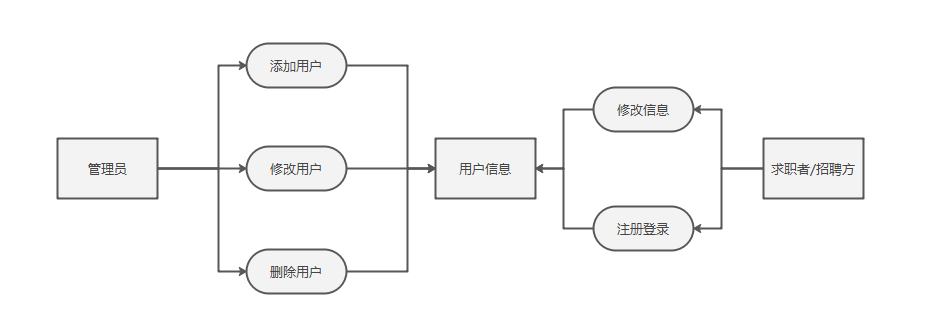
\includegraphics[width=\textwidth]{img/用户信息数据流图.png}
    \caption{用户信息数据流图}
    \label{fig:用户信息数据流图}
\end{figure}

职位信息数据流图如下:

\begin{figure}[H]
    \centering
    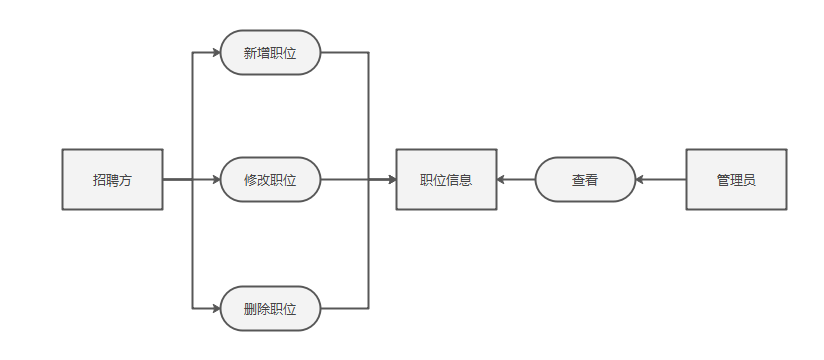
\includegraphics[width=\textwidth]{img/职位信息数据流图.png}
    \caption{职位信息数据流图}
    \label{fig:职位信息数据流图}
\end{figure}

求职信息数据流图如下:

\begin{figure}[H]
    \centering
    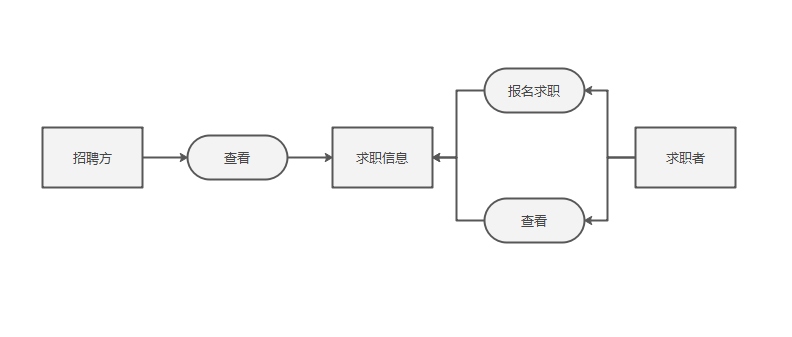
\includegraphics[width=\textwidth]{img/求职信息数据流图.png}
    \caption{求职信息数据流图}
    \label{fig:求职信息数据流图}
\end{figure}

聊天记录信息数据流图如下:

\begin{figure}[H]
    \centering
    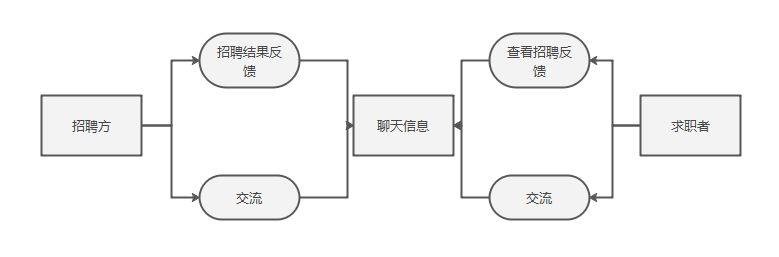
\includegraphics[width=\textwidth]{img/聊天信息数据流图.png}
    \caption{聊天记录信息数据流图}
    \label{fig:聊天信息数据流图}
\end{figure}

\subsubsection{数据字典}

\textbf{(1) 求职者信息表}\\
\begin{center}
\begin{tabular}{|l|l|l|}
\hline
\textbf{字段名} & \textbf{描述} & \textbf{数据类型和约束} \\
\hline
求职者 ID & 唯一标识符,自增长 & - \\
求职者姓名 & 字符串,最大长度为 50 & - \\
性别 & 字符串,最大长度为 10 & - \\
\hline
\end{tabular}
\end{center}

\textbf{(2) 招聘方信息表}\\
\begin{center}
\begin{tabular}{|l|l|l|}
\hline
字段名 & 描述 & 数据类型和约束 \\
\hline
招聘方 ID & 唯一标识符,自增长 & - \\
招聘方姓名 & 字符串,最大长度为 50 & - \\
性别 & 字符串,最大长度为 10 & - \\
\hline
\end{tabular}
\end{center}

\textbf{(3) 管理员信息表}\\
\begin{center}
\begin{tabular}{|l|l|l|}
\hline
字段名 & 描述 & 数据类型和约束 \\
\hline
管理员 ID & 唯一标识符,自增长 & - \\
管理员姓名 & 字符串,最大长度为 50 & - \\
性别 & 字符串,最大长度为 10 & - \\
联系方式 & 字符串,最大长度为 ... & - \\
\hline
\end{tabular}
\end{center}

\textbf{(4) 职位信息表}\\
\begin{center}
\begin{tabular}{|l|l|l|}
\hline
字段名 & 描述 & 数据类型和约束 \\
\hline
职位 ID & 唯一标识符,自增长 & - \\
\hline
\end{tabular}
\end{center}

\textbf{(5) 求职信息表}\\
\begin{center}
\begin{tabular}{|l|l|l|}
\hline
字段名 & 描述 & 数据类型和约束 \\
\hline
报名 ID & 唯一标识符,自增长 & - \\
求职者 ID & 外键,关联求职者信息表中的求职者 ID & - \\
职位 ID & 外键,关联职位信息表中的职位 ID & - \\
\hline
\end{tabular}
\end{center}

\textbf{(6)聊天信息记录表}\\
% 表格结构根据实际字段信息填写

\subsection{功能需求}
功能划分为以下四个部分:
\begin{enumerate}
    \item \textbf{用户管理模块}
    \begin{itemize}
        \item \textbf{用户注册和登录:} 求职者、招聘方和管理员可以通过系统注册账号,并填写个人信息。注册完成后可通过账号和密码登录系统。
        \item \textbf{个人信息管理:} 用户可以查看和修改自己的个人信息,包括姓名、联系方式等。
        \item \textbf{用户权限管理:} 管理员可以设置不同用户的权限,确保各类用户只能访问和操作相应的功能。
    \end{itemize}
    
    \item \textbf{求职者功能模块}
    \begin{itemize}
        \item \textbf{职位浏览和搜索:} 求职者可以浏览和搜索招聘信息,按职位类别、公司、地点等条件筛选职位。
        \item \textbf{简历管理:} 求职者可以在线创建、编辑和管理简历,上传附件等。
        \item \textbf{职位申请:} 求职者可以投递简历至感兴趣的职位,并查看申请状态。
        \item \textbf{职位推荐:} 系统根据求职者的简历和求职意向,推荐适合的职位信息。
    \end{itemize}
    
    \item \textbf{招聘方功能模块}
    \begin{itemize}
        \item \textbf{职位发布和管理:} 招聘方可以发布招聘信息,编辑职位描述,设定招聘要求等。
        \item \textbf{简历筛选和管理:} 招聘方可以浏览和筛选求职者的简历,标记关注简历并管理面试安排。
        \item \textbf{面试通知和反馈:} 招聘方可以发送面试通知,记录面试反馈,并通知求职者录用结果。
    \end{itemize}
    
    \item \textbf{管理员功能模块}
    \begin{itemize}
        \item \textbf{用户账号管理:} 管理员可以审核求职者和招聘方的注册申请,启用或禁用账号。
        \item \textbf{系统监控和维护:} 管理员可以监控系统运行状态,进行维护和更新,确保系统稳定和安全。
        \item \textbf{内容审核:} 管理员审核职位信息,确保招聘信息的合法性和真实性。
        \item \textbf{数据统计和报告:} 管理员生成系统使用报告和统计数据,为决策提供参考。
    \end{itemize}
\end{enumerate}

\subsection{性能/非功能需求}

\begin{enumerate}
    \item \textbf{准确性}:系统应能够支持大量用户同时在线,且响应时间不超过3秒。它应能迅速处理聊天消息传递、报名结果反馈,同时保持24小时的高稳定性运行。
    
    \item \textbf{及时性}:系统应迅速响应用户操作,大多数操作的响应时间应保持在3秒以内。
    
    \item \textbf{可用性}:系统应易于理解并操作,具有友好的用户界面。它应能自适应不同设备和屏幕尺寸,并保证在各种设备上正常运行。此外,系统应具有高可用性和可靠性,防止系统崩溃或数据丢失。
    
    \item \textbf{安全性}:用户密码在输入时应显示为加密状态,并使用pbkdf2\_sha256算法进行加密传输和存储,以确保数据的保密性和完整性。系统应具备用户身份验证和授权机制,防止未授权访问。用户职责应明确区分,以防止越权操作,确保数据安全。系统还应具备防护恶意攻击和数据泄露的能力,以维护系统安全。
    
    \item \textbf{可靠性}:系统应具备数据备份和恢复功能,以防数据丢失。应有故障自动检测和恢复机制,确保系统在故障时能迅速恢复。同时,系统应有日志记录和审计功能,以追踪和监控系统操作。
    
    \item \textbf{易维护性}:系统应具备可扩展性,方便添加新功能和模块。应有可配置性,便于进行系统配置和参数调整。代码结构和文档应易于维护,以便于系统升级和维护。
    
    \item \textbf{标准性}:软件产品应严格依据软件标准进行测试,以确保产品符合质量标准。
    
    \item \textbf{先进性}:系统设计应采用前沿的架构和技术,以满足当前和未来一段时间的系统需求。
\end{enumerate}

\section{系统设计}

\subsection{用例图}

用例图如下图所示
\begin{figure}[H]
    \centering
    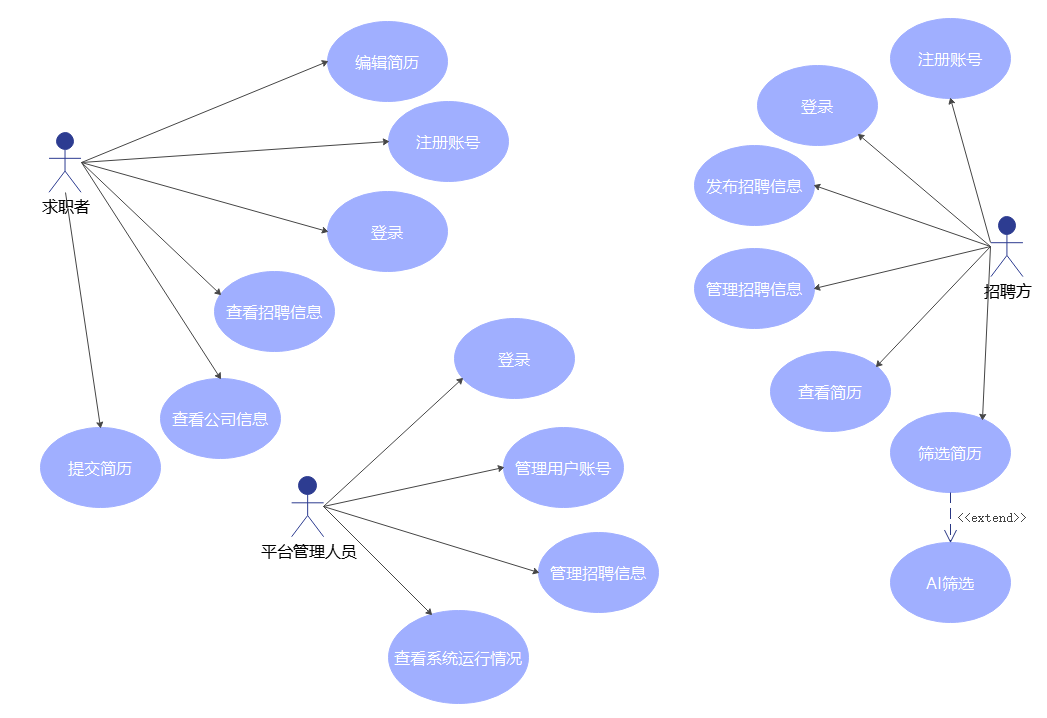
\includegraphics[width=\textwidth]{img/用例图.png}
    \caption{用例图}
    \label{fig:用例图}
\end{figure}

\subsection{活动图}

这一部分,我们用活动图描述两类核心操作:招聘方的招聘操作与求职者的求职操作。其中,求职者的求职操作包括:求职者填写简历;求职者查看招聘信息;求职者投递简历。

\begin{figure}[H]
    \centering
    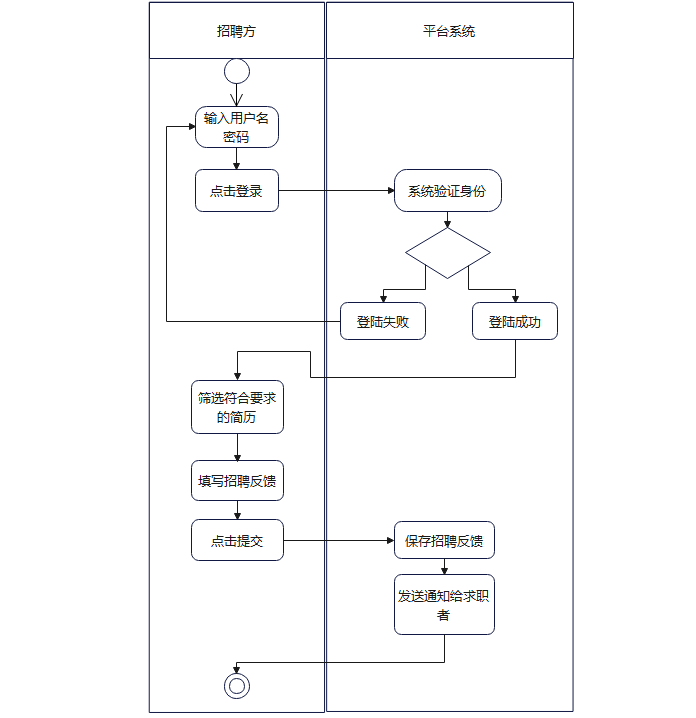
\includegraphics[width=\textwidth]{img/招聘方招聘活动图.png}
    \caption{招聘方招聘活动图}
    \label{fig:招聘方招聘活动图}
\end{figure}

通过活动图可以得到招聘方招聘的过程如下:

\begin{enumerate}
    \item \textbf{招聘方登录:} 首先,招聘方需要在平台系统上进行登录操作。
        \begin{itemize}
            \item 输入用户名和密码。
            \item 点击登录后,系统会进行身份验证。
        \end{itemize}
    
    \item \textbf{系统验证身份:} 根据招聘方提供的用户名和密码,系统会进行身份验证。
        \begin{itemize}
            \item 如果验证失败,则会显示“登陆失败”。
            \item 如果验证成功,则会显示“登陆成功”。
        \end{itemize}
    
    \item \textbf{筛选简历:} 一旦登录成功,招聘方可以进行简历的筛选工作。
        \begin{itemize}
            \item 招聘方需要筛选出符合职位要求的简历。
        \end{itemize}
    
    \item \textbf{填写招聘反馈:} 筛选简历后,招聘方需要填写对候选人的招聘反馈。
        \begin{itemize}
            \item 这可能包括对候选人的评价、面试结果等信息。
        \end{itemize}
    
    \item \textbf{提交和保存招聘反馈:} 填写完招聘反馈后,招聘方需要点击提交。
        \begin{itemize}
            \item 提交后,系统会保存这些招聘反馈。
        \end{itemize}
    
    \item \textbf{发送通知给求职者:} 最后,系统会根据招聘方的反馈,发送相应的通知给求职者。
        \begin{itemize}
            \item 这可能包括面试结果、录用通知或其他相关信息。
        \end{itemize}
\end{enumerate}

\begin{figure}[H]
    \centering
    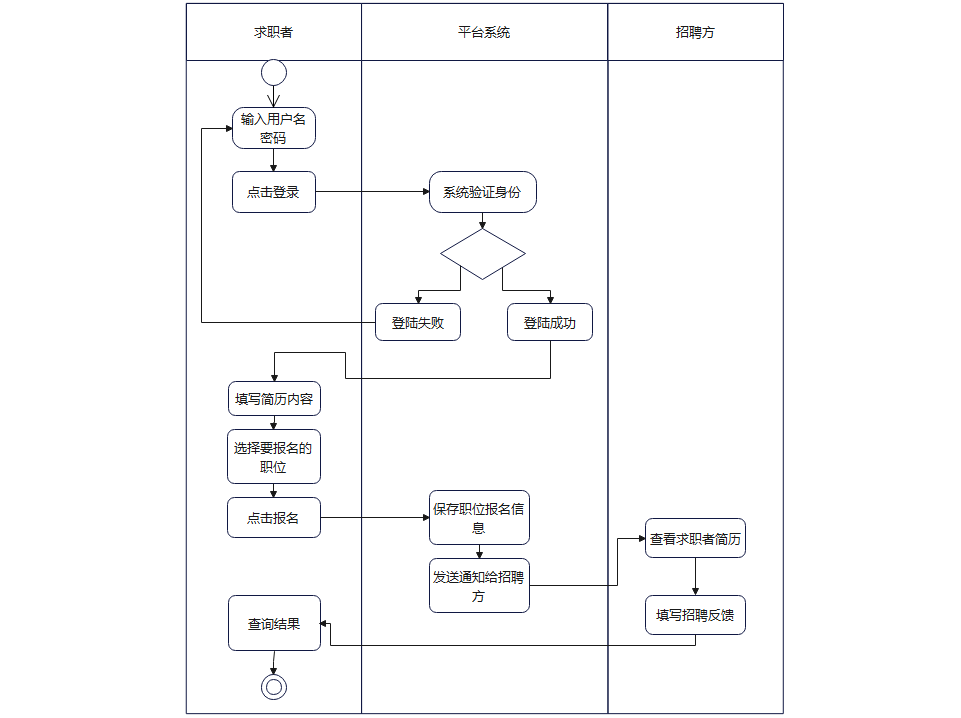
\includegraphics[width=\textwidth]{img/求职者求职活动图.png}
    \caption{求职者求职活动图}
    \label{fig:求职者求职活动图}
\end{figure}

通过活动图可以得到求职者求职的过程如下:

\begin{enumerate}
    \item \textbf{求职者登录:}
        \begin{itemize}
            \item 首先,求职者需要输入用户名和密码。
            \item 接着,求职者点击登录按钮。
        \end{itemize}
    
    \item \textbf{平台系统验证:}
        \begin{itemize}
            \item 系统会验证求职者的身份。
            \item 如果身份验证失败,求职者将无法登录。
            \item 如果身份验证成功,求职者将登陆成功。
        \end{itemize}
    
    \item 登陆成功后,\textbf{求职者操作:}
        \begin{itemize}
            \item 填写简历内容。
            \item 选择想要报名的职位。
            \item 点击报名按钮。
        \end{itemize}
    
    \item \textbf{平台系统响应:}
        \begin{itemize}
            \item 保存职位报名信息。
            \item 发送通知给招聘方。
        \end{itemize}
    
    \item \textbf{招聘方反馈:}
        \begin{itemize}
            \item 招聘方可以查询求职者的报名信息和简历。
            \item 招聘方填写招聘反馈。
        \end{itemize}
\end{enumerate}

\subsection{类图}

(此小节存在过时内容,待进一步交流后更新!)

根据需求,绘制类图如下所示

\begin{figure}[H]
    \centering
    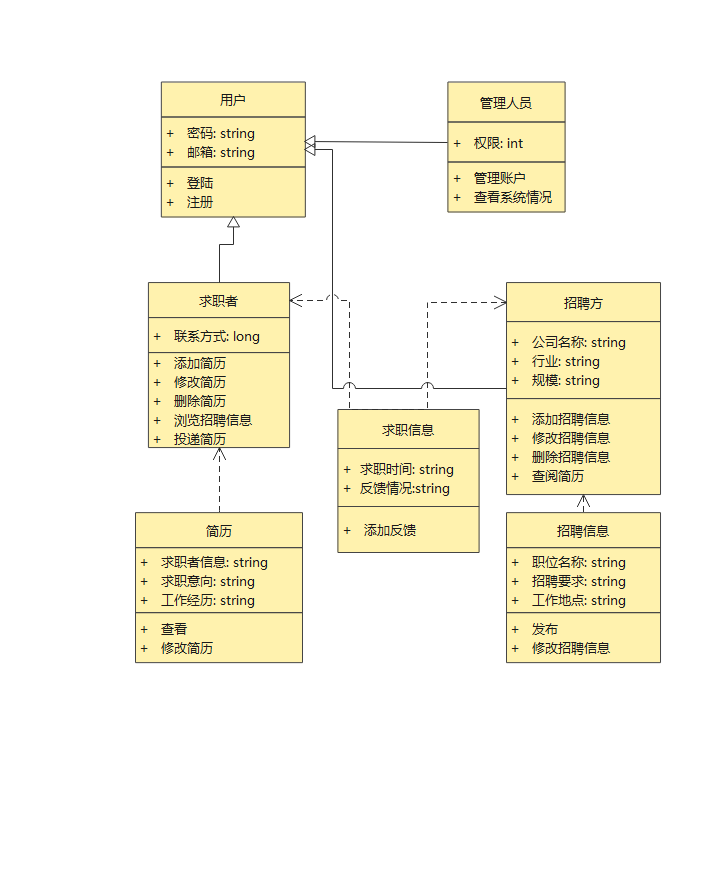
\includegraphics[width=350pt]{img/类图.png}
    \caption{类图}
    \label{fig:类图}
\end{figure}

\subsection{时序图}

我们为招聘方的职位管理功能绘制时序图。这张时序图描述了招聘方用户在使用招聘系统时,进行职位管理的一系列操作流程:

\begin{figure}[H]
    \centering
    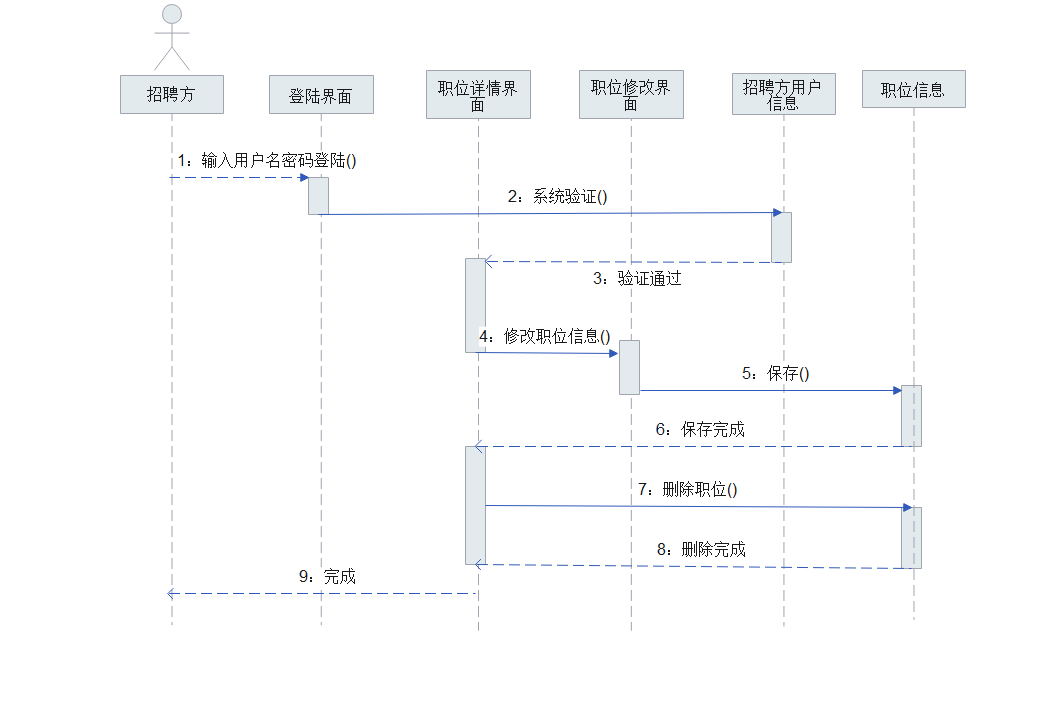
\includegraphics[width=\textwidth]{img/招聘方职位管理时序图.png} 
    \caption{招聘方职位管理操作流程时序图}
    \label{fig:招聘方职位管理时序图}
\end{figure}

以下是时序图中描述的操作步骤:

\begin{enumerate}
    \item \textbf{登录系统:} 招聘方首先登录系统。
    \item \textbf{系统验证:} 系统对招聘方登录信息进行校验。
    \item \textbf{职位管理:} 招聘方进入职位管理界面,进行职位信息的查看、修改或删除。
    \item \textbf{保存修改:} 招聘方修改职位信息后,点击保存。
    \item \textbf{完成操作:} 系统显示操作完成提示,职位信息更新或职位删除成功。
\end{enumerate}

\subsection{协作图——暂无}

\subsection{状态图}

由于招聘、求职过程都围绕着职位展开,因此我们为职位绘制状态图,它描述了一个职位从创建到删除的整个生命周期,如下所示:

\begin{figure}[H]
    \centering
    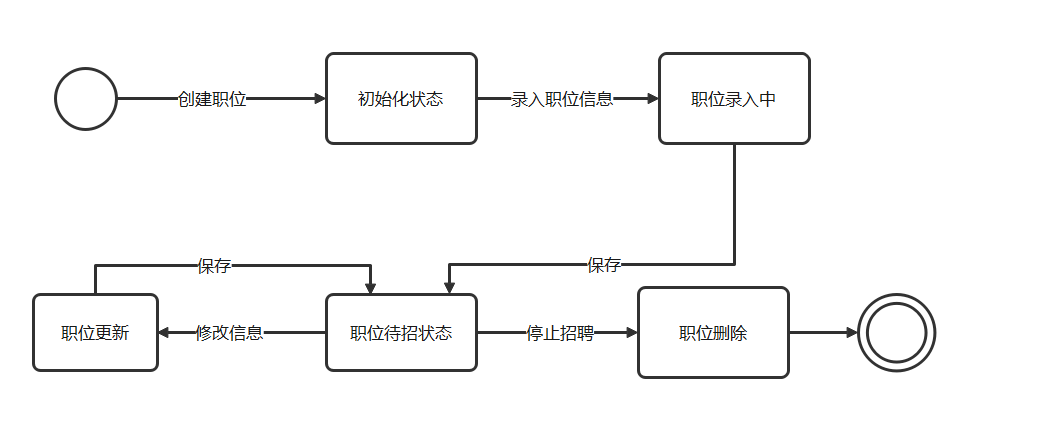
\includegraphics[width=\textwidth]{img/职位状态图.png} 
    \caption{职位生命周期状态图}
    \label{fig:职位状态图}
\end{figure}

以下是状态图中描述的职位生命周期的主要步骤:

\begin{enumerate}
    \item \textbf{创建职位:} 这是职位生命周期的起始点,表示一个新职位的创建过程开始。
    \item \textbf{初始化状态:} 在创建职位之后,系统会进入一个初始化状态,可能用于设置一些基本的参数或默认值。
    \item \textbf{录入职位信息:} 在初始化之后,需要录入具体的职位信息,如职位名称、要求、薪资范围等。
    \item \textbf{职位录入中:} 表示正在录入职位信息的过程。
    \item \textbf{保存:} 录入完职位信息后,可以保存这些信息,使之成为正式的职位记录。
    \item \textbf{职位更新:} 当需要对职位信息进行更改时,可以进入职位更新状态,允许修改已有的职位信息。
    \item \textbf{修改信息:} 在职位更新状态下,可以修改职位的详细信息。
    \item \textbf{职位待招状态:} 表示职位已经准备好,正在等待合适的候选人申请。
    \item \textbf{删除职位:} 如果职位不再需要招聘或已经招到合适的人选,可以进入删除职位状态,准备将职位从系统中移除。
\end{enumerate}

\subsection{构件图——暂无}

\subsection{部署图}

部署图详细展示了系统在物理层面的运行架构,包括硬件的布局以及软件如何在硬件上进行部署。

\begin{figure}[H]
    \centering
    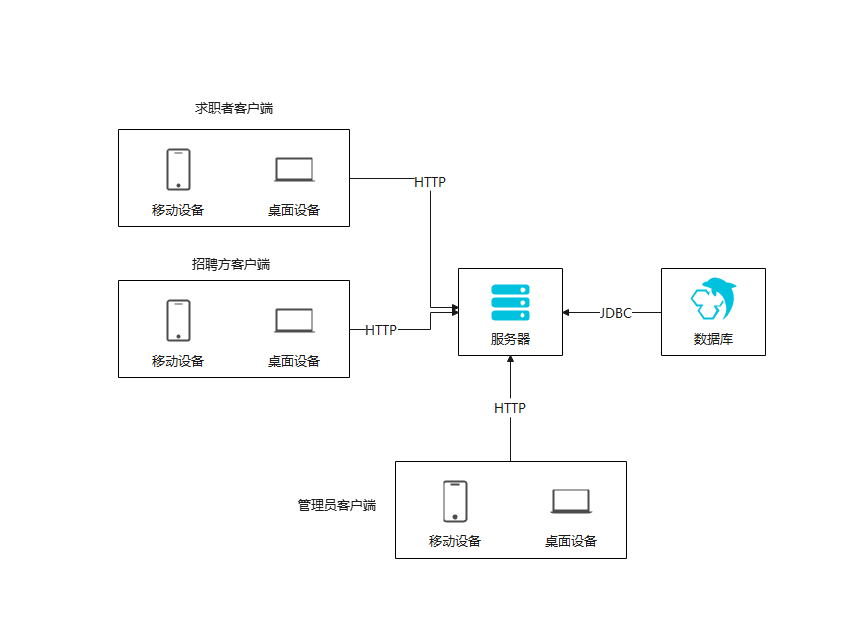
\includegraphics[width=\textwidth]{img/部署图.png} 
    \caption{部署图}
    \label{fig:部署图}
\end{figure}

本系统采用集中式架构设计,从图中可以清晰地识别出硬件的配置和软件部署的详细流程:
- 求职者、招聘方和管理员端均能通过网页浏览器,利用HTTP协议通过互联网访问到Web服务器;
- Web服务器通过JDBC接口与数据库进行交互,实现数据的存储和检索;同时,通过输入输出操作与IO设备进行数据交换。

\section{UI设计}

在交互设计中,需要实现页面之间跳转的设计。在访问网站的时候,首先访问登录注册页面。用户根据自己的角色选择对应的登陆注册界面进行注册、登录,并根据自己登录的角色跳转到对应的首页。求职者身份会跳转到求职者首页,在求职者首页包含职位市场、个人简历、聊天消息等页面入口,在页面内部会包含相应的具体功能。招聘方身份会跳转到招聘方首页,在招聘方首页包含职位发布、公司信息、聊天消息的页面入口,在页面内部会包含相应的具体功能。管理员身份会跳转到管理员首页,管理员包含人员管理(管理求职者和招聘方)、内容审核管理功能页面用于管理职位内容。

\begin{figure}[H]
    \centering
    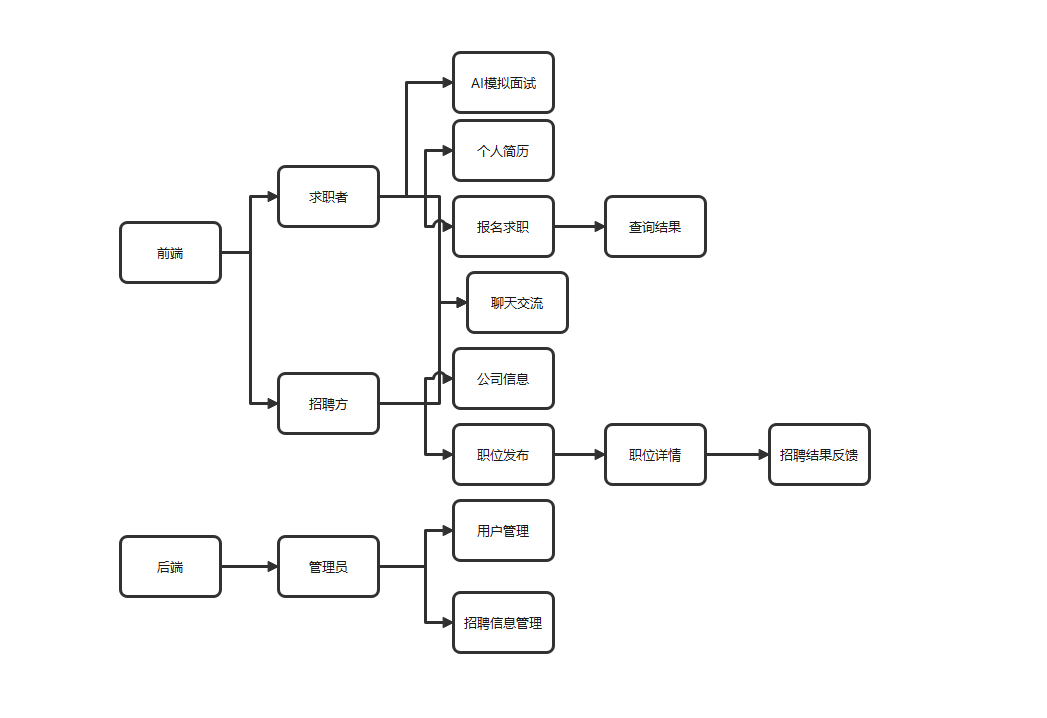
\includegraphics[width=\textwidth]{img/UI交互设计.png} 
    \caption{UI交互设计}
    \label{fig:UI交互设计}
\end{figure}

\section{系统测试}

% 交由负责测试的同学书写

\section{用户手册}

\subsection{引言}

\subsubsection{编写目的}

本章节旨在确立招聘网站的用户需求,明确这些需求在软件实现中的具体形态,以确保软件开发团队和用户对需求有一致且清晰的理解。本章向用户提供了一份详尽的招聘网站使用指南,包括功能、界面和操作的全面解释,旨在帮助用户深入理解并正确使用该软件。此外,本章还提供了逐步指导,以协助新用户迅速掌握软件功能和界面,降低学习成本。


\subsubsection{背景}
\begin{enumerate}
    \item 本用户手册所描述的软件系统的名称为:招聘网站 
    \item 本软件项目的提出者:  
    \item 本软件项目的开发者:  
    \item 本软件项目的目标用户:所有需要招聘和求职的互联网使用者 
\end{enumerate}

\subsubsection{定义}
\textbf{招聘网站}是一个在线平台,它为求职者和雇主提供了一个便捷的互动空间。在这个平台上,求职者可以上传和更新他们的简历,利用关键词、行业类别、工作地点等条件来搜索和申请他们感兴趣的职位。同时,雇主则可以发布职位信息,展示公司文化和工作环境,吸引合适的候选人。招聘网站可以根据用户的求职偏好来推荐职位,提高求职效率。

\subsubsection{参考资料}
\begin{enumerate}
    \item  \href{http://images.china-pub.com/ebook40001-45000/41206/ch01.pdf}{\textit{《软件工程—实践者的研究方法》} Roger S.Pressman, Bruce R.Maxim 编著}
    \item \href{https://www.antpedia.com/standard/74250-1.html}{\textit{《用户手册 GB8567-88 国家标准》}}
    \item \href{http://www.tup.tsinghua.edu.cn/booksCenter/book_08468901.html}{\textit{人机交互: 以用户为中心的设计和评估(第6版)}}
\end{enumerate}

\subsection{用途}

\subsubsection{功能}

此处仅介绍主要功能,更多详细界面功能演示见演示视频。

。。。。图片待前端的同学补充。。。。

\textbf{求职者端}
\begin{enumerate}
    \item 注册功能:求职者输入自己的个人信息,拖动滑块进行注册,注册成功会显示提示弹窗。
    \item 登录功能:求职者输入自己的个人信息,拖动滑块进行登录,登录成功会显示提示弹窗。
    \item 个人信息修改功能:求职者登录之后可在个人中心实现个人信息的修改,修改密码等操作。
    \item 简历修改功能:求职者登录之后可在简历页面修改简历内容并保存。
    \item 报名求职功能:求职者可以在职位市场页面选择理想的职位,报名求职并提交简历。
    \item 求职结果查询功能:求职者求职后可在职位详情页查看求职结果,结果由招聘方反馈,求职结果会在聊天页面同步通知。
    \item 聊天功能:求职者登录之后可在聊天页面与招聘方、其他求职者交流,支持文字和图片形式。
    \item 模拟面试功能:求职者登录之后可在聊天页面选择AI助手进行模拟面试,帮助提升面试技巧。
    % 图片待前端的同学补充
    % ... 其他功能 ...
\end{enumerate}

\textbf{招聘方端}
\begin{enumerate}
    \item 登录功能:招聘方由管理员统一录入信息,输入个人信息,拖动滑块进行登录,登录成功会显示提示弹窗。
    \item 个人信息修改功能:招聘方登录之后可在个人中心实现个人信息的增删改查,修改密码等操作。
    \item 公司信息功能:招聘方登录之后可在公司信息页面实现修改公司的信息。
    \item 职位管理功能:招聘方进入职位发布界面,可以填写职位信息并发布。已发布的职位可以进入详情页面,进一步修改信息或在招聘结束后删除职位。
    \item 招聘功能:招聘方进入职位详情界面,可以查看投递的简历,可以筛选出符合要求的简历,选择合适简历后反馈面试信息,并对剩余简历批量回复婉拒消息。    
\end{enumerate}

\textbf{管理员端}
\begin{enumerate}
    \item 登录功能:管理员输入个人信息,拖动滑块进行登录,登录成功会显示提示弹窗。若忘记密码可以点击界面底部提示,向邮箱发送邮件进行找回。
    \item 个人信息增删改查功能:管理登录之后可在个人中心实现个人信息的增删改查,修改密码等操作。同时它还可以增删改查求职者、招聘方的个人信息和权限。
\end{enumerate}

\subsubsection{性能}

\textbf{(1)精度}\\
本项目的数据包括求职者数据、招聘方数据、职位数据、求职数据、聊天记录数据。其中求职者数据由个人基本数据、简历数据构成,招聘方数据由个人基本数据、公司信息数据构成。其精度说明如下:

\begin{itemize}
    \item 求职者数据
        \begin{itemize}
            \item 姓名:字符串类型,通常是以中文字符表示。
            \item 身份证号码:字符串类型,需符合身份证号码的格式要求。
            \item 性别:字符类型,通常是“男”或“女”。
            \item 出生日期:日期类型,通常以“YYYY-MM-DD”的格式表示。
           % ... 待后端的同学补充...
        \end{itemize}
    \item 招聘方数据
    % ... 待后端的同学补充...
    \item 职位数据
    % ... 待后端的同学补充...
    \item 求职数据
    % ... 待后端的同学补充...
    \item 聊天记录数据
    % ... 待后端的同学补充...
\end{itemize}

\textbf{(2)时间特性}\\
招聘网站时间特性如下:

\begin{itemize}
    \item \textbf{响应时间} \space 所有功能的响应时间应在 1 到 2 秒内。
    \item \textbf{更新处理时间} \space 基于系统规范的设计,软件更新、修复的复杂性较低,软件更新的打包、发布过程相对简单,因此更新处理时间短,较为迅速。
    \item \textbf{数据传输时间} \space 软件数据源存储在本地,故软件具有较快的数据传输时间。为保证软件具有良好的用户体验,所有功能的实现在保证安全性和正确性的情况下,应将响应时间降到最低。
\end{itemize}

\textbf{(3)灵活性}\\
当需求发生某些变化时,招聘网站对这些变化的适应能力的具体情况如下:

\begin{itemize}
    \item 操作方式的变化 本软件具有非常清晰的编程框架与结构,能够很好地应对操作方式需求的变化,例如从网页版调整为手机界面操作软件。
    \item 运行环境变化 本软件能够在 64-bit Windows 10 及以上版本操作系统中运行。
    \item 对软件需求的变化 本软件编程结构清晰,面对用户对软件功能需求的变化能够拥有足够的灵活性,适应需求变化所带来的不同场景和要求。
    \item 时间特性 运行环境的改变不影响软件的响应时间以及数据传输速率。
\end{itemize}

\subsubsection{安全保密性}

招聘网站的安全特性包括但不限于以下几点:
\begin{itemize}
    \item 用户密码输入时界面均显示为加密状态,防止窥屏。
    \item 用户密码存储时,采用 \textbf{pbkdf2\_sha256} 算法迭代 180000 次,防止用户密码泄露。
    \item 应用程序应对用户输入进行验证和过滤,以防止恶意输入和攻击,如注入攻击、跨站脚本攻击等。
    \item 三类用户职责分明,用户无法实现越权的任何操作,实现了数据的安全与保密。
\end{itemize}

\subsubsection{运行环境}

\begin{itemize}
    \item 硬设备
    \begin{enumerate}[label=\arabic*.]
        \item 处理器 12th Gen Intel(R) Core(TM) i7-1260P 2.10 GHz
        \item 系统类型 64 位操作系统基于 x64 的处理器
    \end{enumerate}

    \item 支持软件
    \begin{enumerate}[label=\arabic*.]
        \item 操作系统 Linux 20.04
        \item 编译系统 Python 3.6 + Django 3.0 + Node.js 14.0
        \item 浏览器 推荐 Edge、Google、FireFox
    \end{enumerate}

    \item 数据结构  
    % 待后端的同学补充
\end{itemize}

\subsubsection{使用过程}


    \begin{enumerate}
        \item 安装与初始化
        \begin{itemize}
            \item 项目部署环境具体参数
            \begin{enumerate}[label=(\alph*)]
                \item Python 3.6.0
                \item Django 3.3.0
                \item Node.js 14.0
                \item SQLite Studio 3.4.3
            \end{enumerate}
            \item 项目部署流程
            \begin{enumerate}[label=(\roman*)]
                \item 对于项目前端而言:
                \begin{itemize}
                    \item 使用 npm run install 安装依赖
                    \item 使用 npm run serve 运行前端环境
                \end{itemize}
                \item 对于项目后端而言:
                \begin{itemize}
                    \item 使用 pip install -r requirements.txt 安装依赖
                    \item 使用 python manage.py migrate 迁移数据库
                    \item 使用 python manage.py runserver 运行后端环境
                \end{itemize}
            \end{enumerate}
        \end{itemize}
        
        \item 输入输出
        % 待前端的同学补充
        
        \item 文卷查询
        本软件所有用户数据、职位数据、求职数据都是基于软件的所有查询操作,无需用户额外输入查询参数。用户参数在用户登录时获取完成,采用隐式传参的方式在服务器端进行执行数据的查询。由于软件数据以数据库基表的形式进行存储,所以数据查询本质上采用 SQL 语句完成。
        
        \item 出错处理和恢复
        软件客户端在正常运行的下,一般不会出现问题。多数问题出现在服务端,当服务器端无法访问,或服务端运行崩溃时,将短暂关闭服务器端。在关闭服务端后,用户使用软件会获取到服务无法访问等相关提示。当软件出现卡顿,崩溃等情况,强制关闭即可。服务端会在修复后进行重启,用户重启软件即可正常使用服务。为保证系统的稳定性,我们会定期进行压力测试,稳定性测试,确保用户能够及时获取服务。
        
        \item 终端操作
        本软件基于 C/S 模式,采用客户端服务器模式开发,软件在各终端独立运行,无需终端之间连接,各终端与服务器独立通信。终端在进行修改操作时,服务器采用事务处理原则,遵从事务处理原子性,保证用户数据的准确性。服务器具有一定的并行能力,支持多终端同时访问。
    \end{enumerate}
    
\section{项目部署环境具体参数}

\subsection{项目语言}
以 Python 语言为主,涉及 JavaScript、CSS、Vue 13.3、HTML 等。

\subsection{项目框架}
使用 Django+Vue 框架,前后端分离。其中 Django 主要实现后端,Vue 主要实现前端。

\subsection{引用包的具体版本}
\begin{enumerate}
    \item Python 3.6.0
    \item Django 3.3.0
    \item Node.js 14.0
    \item SQLite Studio 3.4.3
\end{enumerate}

其余依赖包的具体版本如下所示 (\texttt{requirements.txt}):
\begin{framed}
\begin{verbatim}
asgiref==3.2.3
certifi==2019.11.28
chardet==3.0.4
coreapi==2.3.3
coreschema==0.0.4
defusedxml==0.6.0
diff-match-patch==20181111
Django==3.0.3
django-crispy-forms==1.9.0
django-filter==2.2.0
django-formtools==2.2
django-guardian==2.2.0
django-import-export==2.0.2
django-reversion==3.0.7
djangorestframework==3.11.0
djangorestframework-jwt==1.11.0
et-xmlfile==1.0.1
future==0.18.2
httplib2==0.9.2
idna==2.9
itypes==1.1.0
jdcal==1.4.1
Jinja2==2.11.1
MarkupPy==1.14
MarkupSafe==1.1.1
odfpy==1.4.1
openpyxl==3.0.3
PyJWT==1.7.1
pytz==2019.3
PyYAML==5.3
requests==2.23.0
sqlparse==0.3.1
tablib==1.1.0
uritemplate==3.0.1
urllib3==1.25.8
xadmin2==2.0.3
xlrd==1.2.0
xlwt==1.3.0
\end{verbatim}
\end{framed}

\subsection{项目安装部署流程}

\begin{enumerate}
    \item 对于项目前端而言:
    \begin{enumerate}
        \item 使用 \texttt{npm run install} 安装依赖
        \item 使用 \texttt{npm run serve} 运行前端环境
    \end{enumerate}
    \item 对于项目后端而言:
    \begin{enumerate}
        \item 使用 \texttt{pip install -r requirements.txt} 安装依赖
        \item 使用 \texttt{python manage.py migrate} 迁移数据库
        \item 使用 \texttt{python manage.py runserver} 运行后端环境
    \end{enumerate}
\end{enumerate}

% 此外我们还将本地网址上传至服务器,短时间内可通过以下网址访问:
% \begin{itemize}
%     \item 前端:http://172.96.160.54/
%     \item 后端:http://172.96.160.54/xadmin/
% \end{itemize}

\section{项目GitHub地址}

\url{https://github.com/want6to6good/softwore-work/tree/main}

\section{项目功能截图}

项目具体功能实现的截图见讲解视频,此处不重复叙述。

\section{代码功能介绍}

(交由负责前后端的同学书写)

\section{总结}

在本学期的软件工程大作业中,我和团队共同合作完成了一个招聘平台网站,采用了Django+Vue框架,实现了前后端分离的架构。该平台不仅满足了求职者和招聘方要求的基本功能,如职位发布、简历投递求职、招聘结果反馈等,还针对求职者需求额外设计了大模型模拟面试功能,以便求职者提升面试能力。

我们在项目开发过程中,进行了前期调研分析,编写了前后端单元测试,并完成了功能和性能测试。为了保证用户信息的安全性,我们采用了pbkdf2\_sha256算法进行密码存储。

整个项目开发过程使我们深刻体验到了软件工程的全过程,从需求分析、功能设计、实现、代码合并,到测试和文档撰写等多个环节。这不仅锻炼了我们的软件工程能力,还增强了团队合作意识,收获了知识和友谊。

% ... 其他内容 ...
\end{document}
